\section{Prompts}
\label{appx:prompts}

In this section, we go through the prompt templates that make up the agent’s history, discussing them in the order of presentation to SWE-agent.
Per template, we describe its purpose, walk through its content, and note any additional motivations that influenced how we wrote the template.
The companion figures of template content are all drawn from our default configuration, using SWE-agent w/ GPT-4.

The template content can and should be adapted slightly to fit the agent's intended use case.
The purpose of this section is to describe our thought process for how we designed each template for these tasks to serve as reference for future work.
Across templates, we find that providing tips which tell agents to not make specific mistakes, avoid common pitfalls, and use helpful execution signals are effective for eliciting more successful problem solving.

\textbf{Prompt Workflow.}
We present Figure~\ref{fig.prompt_flow} which shows the order in which different prompt templates are invoked.
This flow of prompts reflects the logic that generates trajectories similar to the one that is visualized in Figure~\ref{fig.trajectory_overview}.

\begin{figure}[ht]
    \centering
    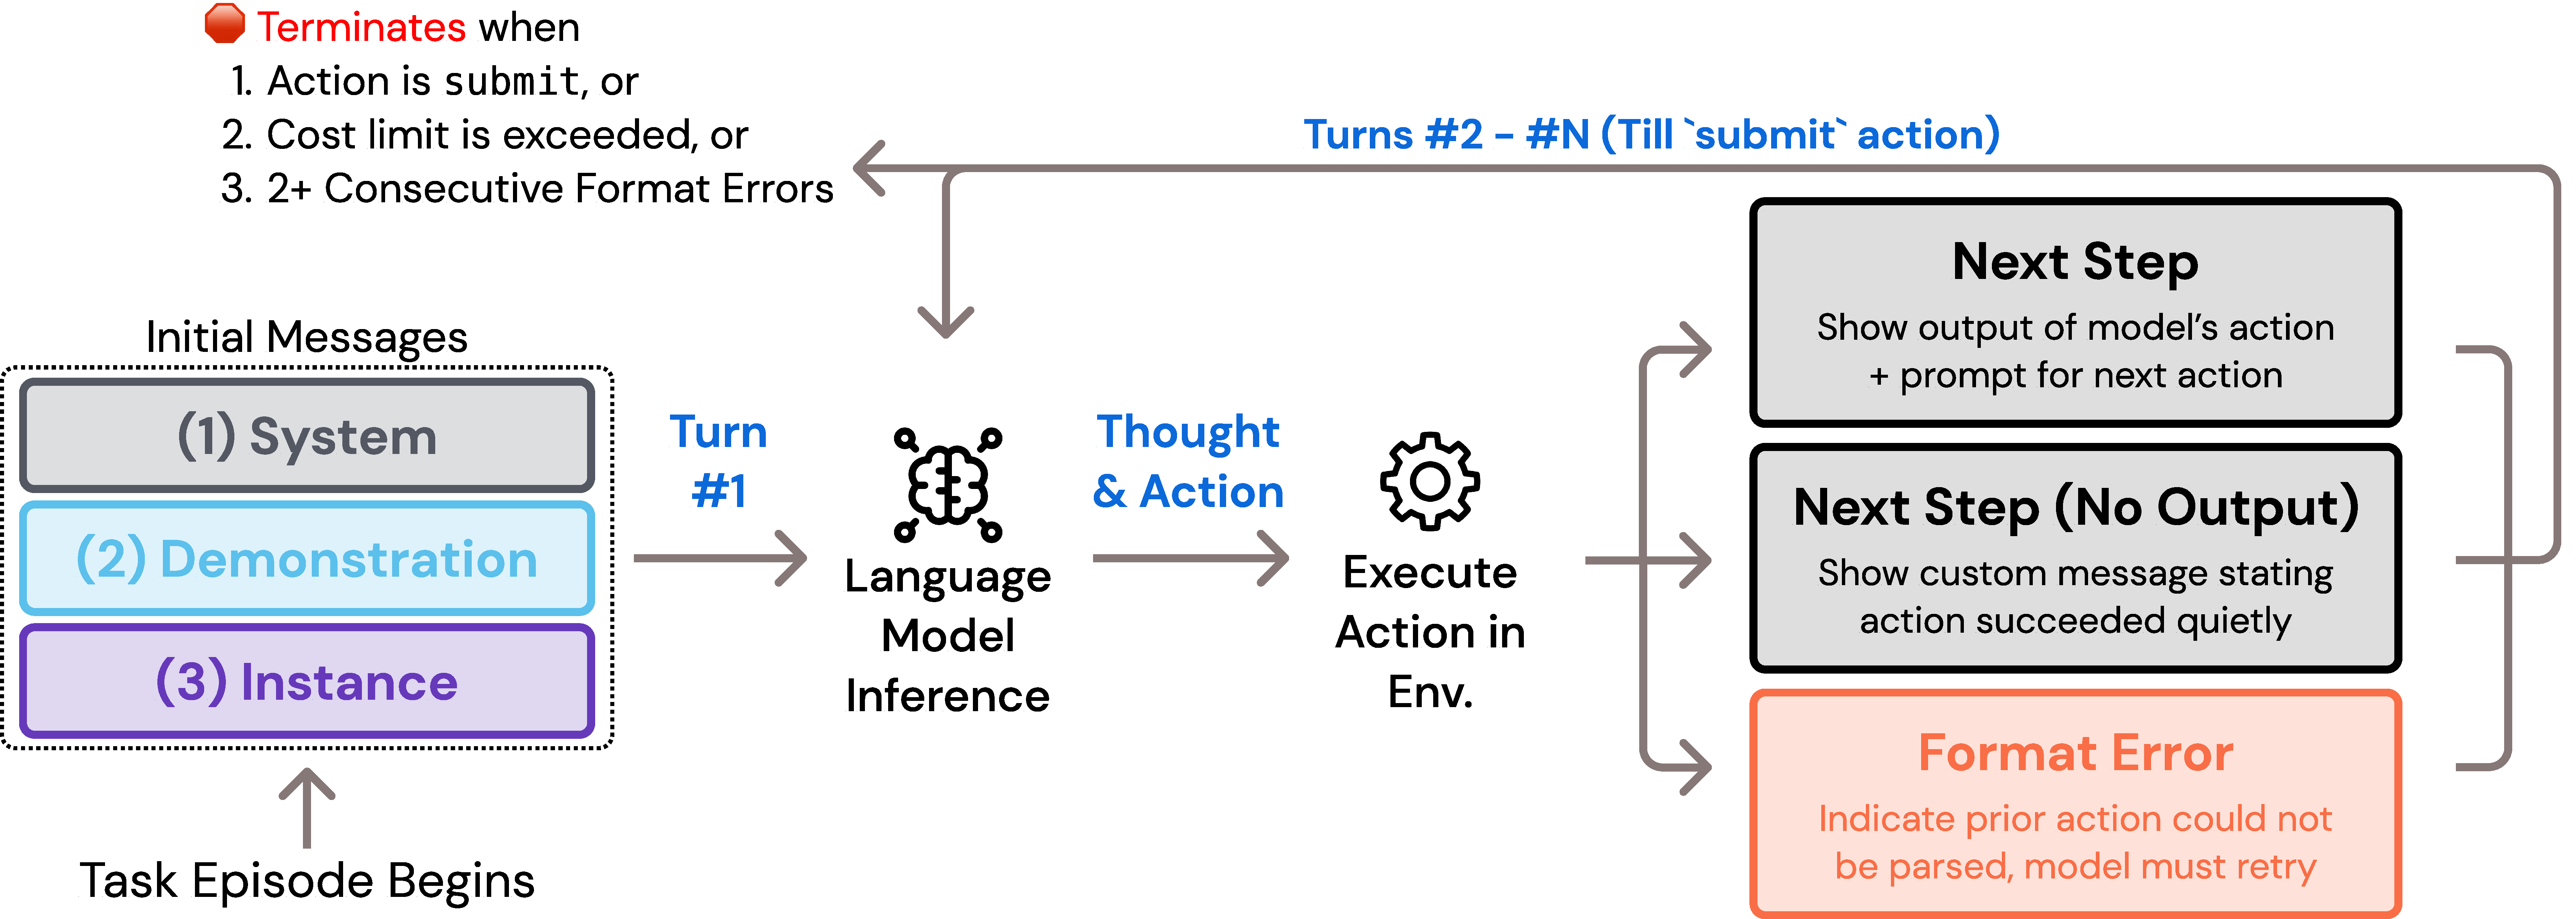
\includegraphics[width=\linewidth]{figures/appx/prompt_flow.pdf}
    \caption{The flow of prompt templates throughout a single SWE-agent task instance episode. The system, demonstration, and issue templates are shown all together at the beginning of the task episode, followed by turn-specific prompts that are shown depending on whether the agent response is well-formatted and whether the action has standard output.}
    \label{fig.prompt_flow}
\end{figure}

\textbf{System Template.}
The system template describes the interactive task setting, the commands at the agent’s disposal, and the expected response format.
It is the first message for any episode, does not change in content across task instances, and is not removed or collapsed at any point from the message history.
The agent is told of the general task setting, which is a command line that comes with a special file viewer interface.
After this, the agent is presented the command documentation, which shows a usage example and docstring for every custom command, mirroring the content of Figure~\ref{fig.prompts.system}.
As discussed before, from manual observation, we find that agents need a lot of support to make effective use of the \texttt{edit} command.

{
\begin{promptbox}{System Prompt}
\textbf{SETTING:} You are an autonomous programmer, and you're working directly in the command line with a special interface.
\smallskip

The special interface consists of a file editor that shows you 100 lines of a file at a time.
In addition to typical bash commands, you can also use the following commands to help you navigate and edit files.
\smallskip

\textbf{COMMANDS:} \{documentation\}
\smallskip

Please note that THE EDIT COMMAND REQUIRES PROPER INDENTATION. 
If you'd like to add the line `\;\;\;\;\;\;\;\;print(x)' you must fully write that out, with all those spaces before the code! Indentation is important and code that is not indented correctly will fail and require fixing before it can be run.
\smallskip

\textbf{RESPONSE FORMAT:} \\
Your shell prompt is formatted as follows: \\
(Open file: \textless{}path\textgreater{}) \textless{}cwd\textgreater{} \$ \\
You need to format your output using two fields; discussion and command.
Your output should always include \textit{one} discussion and \textit{one} command field EXACTLY as in the following example:
\smallskip

DISCUSSION \\
First I'll start by using ls to see what files are in the current directory. Then maybe we can look at some relevant files to see what they look like. \\
\`{}\`{}\`{} \\
ls -a \\
\`{}\`{}\`{} 

\smallskip
You should only include a \textit{SINGLE} command in the command section and then wait for a response from the shell before continuing with more discussion and commands. Everything you include in the DISCUSSION section will be saved for future reference. 
If you'd like to issue two commands at once, PLEASE DO NOT DO THAT! Please instead first submit just the first command, and then after receiving a response you'll be able to issue the second command. 
You're free to use any other bash commands you want (e.g. find, grep, cat, ls, cd) in addition to the special commands listed above. 
However, the environment does NOT support interactive session commands (e.g. python, vim), so please do not invoke them.
\end{promptbox}%
\captionsetup{type=figure}
\captionof{figure}{The system prompt for SWE-agent describes the environment. The \texttt{documentation} field is populated with brief description of all enabled commands, similar to Table \ref{tab:commands}.}
\label{fig.prompts.system}
}


An agent will occasionally generate an \texttt{edit} with either the wrong level of indentation or incorrectly specified line numbers.
Because of this, we include a note telling the agent to pay attention to proper indentation.
% We did not ablate this note, but from our recollection of the early development process, including this text with proper indentation in all caps seems to provide some extra motivation for the agent to get it right.
Finally, the system prompt describes what the agent’s response should look like, communicated with an example (e.g. JSON format, XML delimiters) followed by a paragraph reinforcing the importance of issuing a \textit{single} thought/action pair per turn.
Because of the constraints imposed by Docker containers, we include one last point about the command line environment not supporting any interactive session commands, such as \texttt{vi} or \texttt{python}.
The system template does not introduce any task instance specific information.

\textbf{Demonstration Template.}
If provided, the demonstration template immediately follows the system template as the second message showing the agent a trajectory which resulted in the successful resolution of a task instance from the development set.
As confirmed by the ablation in Table~\ref{tab:combined_ablations_summary}, including a demonstration slightly helps agents with understanding proper command usage and reduces the rate of errant responses.
Rather than being written out entirely like the system template, the demonstration template is put together based on two fields as shown in the configuration file discussed in Section~\ref{appx:interface:configuration}.
First, the \texttt{demonstrations} argument points at 1+ \texttt{.traj} file(s), each containing a multi-turn, SWE-agent style history of interactions.

Second, the \texttt{demonstration\_template} and \texttt{put\_demos\_in\_history} arguments control how the demonstration is represented in the message history.
If the \texttt{put\_demos\_in\_history} argument is set \texttt{True}, every turn of the demonstration trajectory is used as a separate message in the history.
The alternative is to write out the entire demonstration as a single message, wrapped in a natural language instruction indicating it is a demonstration (this is the method that is displayed in Figure~\ref{fig.prompts.demonstration}).
The effectiveness of each method varies by model.
The first method of adding a demonstration as separate messages can be preferable because it gives an agent the impression that it has already solved a task instance and is working on the next one.
However, for a different model, it can be confusing to have the contexts from two tasks in a single trajectory, which is why the second method of explicitly telling the model that it’s being given a demonstration can be better.

{
\begin{fileviewerbox}{Demonstration}
\begin{Verbatim}[breaklines=true]
Here is a demonstration of how to correctly accomplish this task.
It is included to show you how to correctly use the interface.
You do not need to follow exactly what is done in the demonstration.
--- DEMONSTRATION ---
{{INSTANCE PROMPT}}

The code has been updated to use the `round` function, which should fix the rounding issue. Before submitting the changes, it would be prudent to run the reproduce.py code again to ensure that this change has the desired effect. I see that "Current directory" is still `/marshmallow-code__marshmallow`, so we can just run `reproduce.py` directly.
```
python reproduce.py
```
345

(Open file: /marshmallow-code__marshmallow/src/marshmallow/fields.py)
(Current directory: /marshmallow-code__marshmallow)
bash-$
The output has changed from 344 to 345, which suggests that the rounding issue has been fixed. Let's remove the reproduce.py file since it is no longer needed.
```
rm reproduce.py
```
Your command ran successfully and did not produce any output.
(Open file: /marshmallow-code__marshmallow/src/marshmallow/fields.py)
(Current directory: /marshmallow-code__marshmallow)
bash-$
rm doesn't have any output when it deletes successfully, so that must have worked. Now that we have fixed the issue, we should submit our changes to the code base. Let's submit the changes using the `submit` command.
```
submit
```
--- END OF DEMONSTRATION ---
\end{Verbatim}
\end{fileviewerbox}
\captionsetup{type=figure}
\captionof{figure}{
A simplified demonstration template showing how demonstrations are provided to the model as a single message.
Here we show only the final $3$ turns in the demonstration for brevity.
}
\label{fig.prompts.demonstration}
}

We are unsure if demonstrations actually help agents understand the nuances of domain specific problem solving.
Because of the diversity of software engineering issues, we think the role the demonstration plays is primarily to help the agent learn to issue properly formatted commands.
Prior work has demonstrated that fine tuning may have the potential to imbue agents with a certain degree of expertise around how to adaptively solve task instances that may vary in terms of what strategy is most successful.

\textbf{Instance Template.}
The instance template introduces the agent to the task instance.
The problem statement is shown, followed by a brief set of instructions that reiterate important points from the system template.
These points are the one thought/action per-turn requirement, mentioning the lack of support for interactive shell commands, and a reminder of the importance of editing indentation.
Finally, a notably effective part of the instance template is the inclusion of tips which serve as an additional guidelines for how to operate successfully in the bash environment, shown in Figure~\ref{fig.prompts.instance}.
These tips were developed manually and iteratively; after running SWE-agent with a particular configuration on the development set, we manually looked at the trajectories for failure modes.
The tips were born out of these failures, and through repeated inspection, we found that such tips did reduce the frequency of errant problem solving strategies that they are meant to address.
While our manual approach to writing tips certainly does not scale, representing feedback for common mistakes as tips is surprisingly effective.
Developing better methods for this process of identifying failure modes and writing natural language instructions that describe the correct alternative behavior could be an avenue to better performance for future SWE-agent based systems.
Finally, at the end of the message, the agent is presented with a command line prompt indicating that the task has begun and that the agent should issue its first command.

{
\begin{fileviewerbox}{Instance Message}
\begin{Verbatim}[breaklines=true]
We're currently solving the following issue within our repository.
Here's the issue text:
ISSUE:
{issue}

INSTRUCTIONS:
Now, you're going to solve this issue on your own. Your terminal session has started and you're in the repository's root directory. You can use any bash commands or the special interface to help you. Edit all the files you need to and run any checks or tests that you want.  Remember, YOU CAN ONLY ENTER ONE COMMAND AT A TIME. You should always wait for feedback after every command.  When you're satisfied with all of the changes you've made, you can submit your changes to the code base by simply running the submit command. Note however that you cannot use any interactive session commands (e.g. python, vim) in this environment, but you can write scripts and run them. E.g. you can write a python script and then run it with `python <script_name>.py`.

NOTE ABOUT THE EDIT COMMAND: Indentation really matters! When editing a file, make sure to insert appropriate indentation before each line! 

IMPORTANT TIPS:
1. Always start by trying to replicate the bug that the issues discusses. If the issue includes code for reproducing the bug, we recommend that you re-implement that in your environment, and run it to make sure you can reproduce the bug. Then start trying to fix it. When you think you've fixed the bug, re-run the bug reproduction script to make sure that the bug has indeed been fixed.

2. If you run a command and it doesn't work, try running a different command. A command that did not work once will not work the second time unless you modify it!

3. If you open a file and need to get to an area around a specific line that is not in the first 100 lines, say line 583, don't just use the scroll_down command multiple times. Instead, use the goto 583 command. It's much quicker. 
 
4. If the bug reproduction script requires inputting/reading a specific file, such as buggy-input.png, and you'd like to understand how to input that file, conduct a search in the existing repo code, to see whether someone else has already done that. Do this by running the command: find_file "buggy-input.png" If that doesn't work, use the linux 'find' command. 

5. Always make sure to look at the currently open file and the current working directory (which appears right after the currently open file). The currently open file might be in a different directory than the working directory! Note that some commands, such as 'create', open files, so they might change the current  open file.

6. When editing files, it is easy to accidentally specify a wrong line number or to write code with incorrect indentation. Always check the code after you issue an edit to make sure that it reflects what you wanted to accomplish. If it didn't, issue another command to fix it.
 

(Open file: {open_file})
(Current directory: {working_dir})
bash-$
\end{Verbatim}
\end{fileviewerbox}
\captionsetup{type=figure}
\captionof{figure}{
The instance template. This message shows the task instance's problem statement (referenced by the \texttt{\{issue\}} field), shows additional task instance-specific information, and provides a set of tips suggesting recommended problem solving approaches and pitfalls to look out for.
}
\label{fig.prompts.instance}
}

\textbf{Next Step Template.}
Assuming an agent’s response is well formed and contains an action, there are two simple templates used to present the corresponding output of the agent’s action, as shown in Figure~\ref{fig.prompts.next_step}.
If an agent’s action produces some standard output, the agent is simply shown this output with a command line prompt to indicate that the agent should respond with the next action.

{
\captionsetup{type=figure}
\begin{promptbox}{Next Step Template}
\begin{verbatim}
{OBSERVATION}
(Open file: /path/to/open/file.py)
(Current directory: /path/to/cwd)
bash-$
\end{verbatim}
\end{promptbox}
\captionof{figure}{
The environment's ``next step" template.
This is emitted after each observation to inform the model of the current state of the shell and programs.
}
\label{fig.prompts.next_step}
}

However, if an agent’s action runs silently and produces no output (e.g. \texttt{rm abc.py}, \texttt{touch abc.py}), we found that simple showing no output along with a prompt can be confusing for agents to interpret, and it will often run additional, unnecessary commands to determine the effect of the prior action.
To guard against this situation, the agent is informed verbosely that the command ran successfully and did not produce output.
While the System, Demonstration, and Instances template are only used a single time, the next step template is used repeatedly.
In the SWE-agent configuration described in this work, the next step templates are fairly simple, as they essentially just add the command line prompt to the end of the execution standard output.
We have not explored other variations to this style.

\textbf{Collapsed Observation Template.}
As shown in Figure~\ref{fig.trajectory_overview} and discussed in Section~\ref{sec:aci}, old observations are \textit{collapsed}; meaning that the structure and order of the agent's interaction history is preserved, but the content of old observations are replaced with a one-line placeholder.
This summary simply states that the observation is omitted with the number of lines that were removed, as shown in Figure~\ref{fig.prompts.collapsed_obs}.

{
\captionsetup{type=figure}
\begin{promptbox}{Environment Response (collapsed) Template}
\begin{verbatim}
Old output omitted (101 lines)
\end{verbatim}
\end{promptbox}
\captionof{figure}{
A \textit{collapsed} environment response.
The content of old observations are replaced with this template.
}
\label{fig.prompts.collapsed_obs}
}

The purpose of collapsing old observations is twofold.
First, it simply reduces the number of tokens needing to be processed at each interaction step.
Second, by removing old observations' content, it can also reduce the presence of outdated or duplicate information, such as directory and file contents or command output.
We think that both of these purposes can serve to improve agent performance.

\textbf{Error Message Template.}
An agent's response is not always well formed.
As discussed, an agent is generally expected to respond with a single thought and action per turn.
In our work, we experimented with asking the agent to generate one of three different styles of responses for communicating one thought and one action (same type of response across any single episode).

\begin{enumerate}[noitemsep]
    \item A string where the action is wrapped as a markdown-style code block (\`{}\`{}\`{}).
    \item A JSON style dictionary with ``thought" and ``action" keys.
    \item An XML style generation with ``$<$thought$>$" and ``$<$action$>$" delimiters.
\end{enumerate}

On occasion, an agent may generate a response that doesn't conform to the requested format.
If this occurs, we show an error message to the agent indicating that the prior message was malformed and to issue another response that does not make the same mistake, as presented in Figure~\ref{fig.prompts.error}.
If a model generates \num{3} malformed responses in a row, the episode will terminate early.

{
\captionsetup{type=figure}
\begin{promptbox}{Error Message}
\begin{verbatim}
Your output was not formatted correctly. You must always include one
discussion and one command as part of your response. Make sure you do
not have multiple discussion/command tags.
Please make sure your output precisely matches the following format:
DISCUSSION
Discuss here with yourself about what your planning and what you're
going to do in this step.

```
command(s) that you're going to run
```
\end{verbatim}
\end{promptbox}
\captionof{figure}{
The environment's error message.
This is emitted if a model generation doesn't conform to the thought-action format suggested.
}
\label{fig.prompts.error}
}

Another context management trick is that if models generate a malformed response, but then subsequently respond with a valid one, the message history is modified such that the action and response correspond to the malformed generation is removed.
This kind of de-noising reduces unnecessary context and helps prevent future malformed generations.
Each well-formatted response becomes an additional in-context demonstration of how to interact with the environment correctly; this ``momentum'' of correct responses is effective for helping agents continue to issue correct actions at later turns in trajectories when there is a lot of information in the message history.